The overall process for the coordinated voltage control algorithm is shown in Fig. \ref{fig:Overview}, and the 'select supply node' subroutine is shown in \ref{fig:sub_rou}. The different blocks presented in the Fig. \ref{fig:Overview} are as follows:

\begin{figure}[!h]
\centering
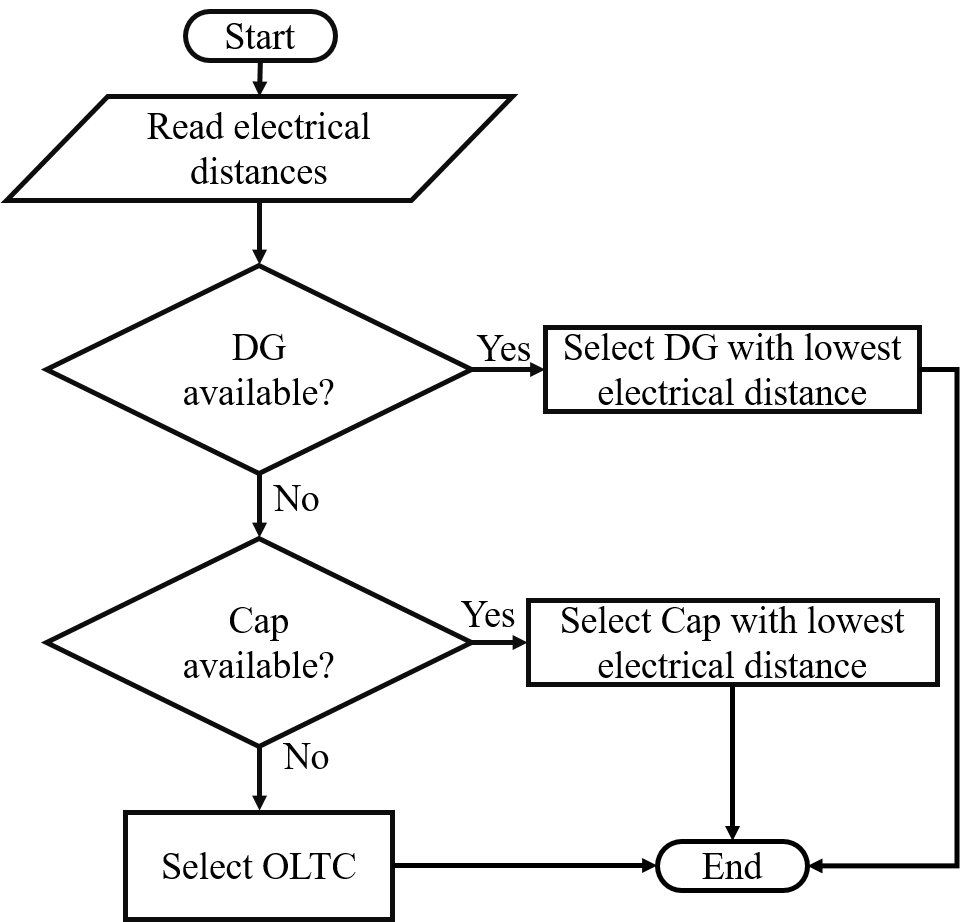
\includegraphics[width=0.8\linewidth]{figs/Flow_chart_2_1.png}
\caption{Select supply node subroutine}
\label{fig:sub_rou}
\end{figure}



\begin{figure}[!h]
\centering
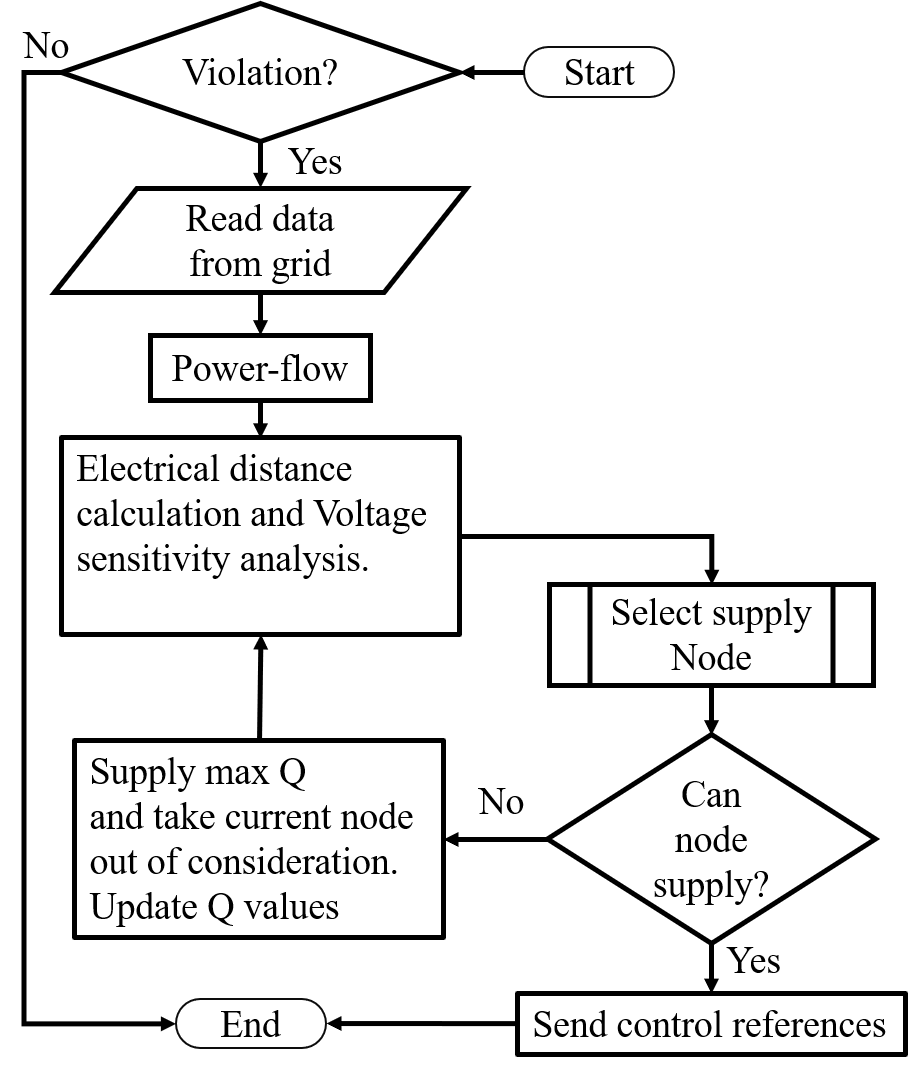
\includegraphics[width=0.8\linewidth]{figs/FLOW_CHART_3.png}
\caption{Flowchart of the proposed CVC scheme}
\label{fig:Overview}
\end{figure}

\begin{enumerate}
    \item \textbf{Violation?:} At the start of the algorithm it checks for a signal from the distribution system to see if a violation has occurred. It is assumed that the distribution system has systems in place to detect voltage violations as the purpose of the algorithm is to coordinate the response of the available resources to mitigate the violation. If there is no violation detected the algorithm does not take any actions. If a violation has occurred the algorithm continues.
    
    \item \textbf{Read data from grid:} In this step the algorithm reads the real power $P$ and reactive power $Q$ demands from all the loads and inverter interfaced DGs in the system. It also receives the status of the capacitor banks (ON/OFF) and the current tap position of any on load tap changer (OLTC) available in the system. And finally it receives voltage magnitude $|V|$ measurements from any points of the system where such measurements are available.
    
    % The distribution grid block represents the actual distribution grid the proposed CVC will be in charge of. The distribution grid will provide the real and reactive power P and Q and the voltage magnitude $|V|$ of all the measured points from the system to the algorithm when a voltage violation is detected.
    % \item \textbf{Bad data detection:} This section will make use of bad data detection algorithms to determine bad data received from the system. This step will filter out the bad data and provide the next step with accurate system data. (This will be the last step developed and might not be included in the IET special issue paper planned to be submitted at FALL 2019).
    \item \textbf{Power-flow:} The power-flow step uses the data acquired in the previous step to estimate the remaining voltage angles and magnitudes of nodes that do not have measurements. 
    
    \item \textbf{Voltage sensitivity analysis and electrical distance calculation:} Using the data from the power-flow, this step the voltage sensitivity analysis and electrical distance calculations will be performed to determine the best node to supply reactive power compensation to aid in voltage regulation. This step also determines how much reactive power compensation should the selected node provide. These concepts have been explained in detail in Section \ref{vsa} and \ref{edc}.
    
    \item \textbf{Select supply node:} This sub routine is shown in \ref{fig:sub_rou}. The sub routine starts by reading the electrical distances from the previous steps. Then it first checks to see if there are any DGs available to supply reactive power in the 'DG available?' step. If there are it selects the DG with the least electrical distance to supply reactive power compensation. Other wise it checks for capacitor banks available if the 'Cap available?' step. If there are capacitor banks available to be turned on or off to tackle the voltage violation the sub routine selects the capacitor bank with the lowest electrical distance. Finally if there are no DG or capacitor banks available, OLTC is selected to mitigate the voltage violation. 
    
    \item \textbf{Can node supply?:} This step checks if the resources available at the selected node has the capability to supply the required reactive power compensation. If it does, the algorithm moves on to the 'Send Q references' step. Otherwise, it goes to the 'Supply max Q and takes current node out of consideration' step.
    
    %the reactive power reference is sent to the actual equipment available at the distribution grid. Otherwise, the algorithm updates the resources at the current node to supply maximum reactive power and sends the updated system status to Voltage sensitivity analysis and electrical distance calculation and the algorithm runs voltage sensitivity analysis and electrical distance calculation again to find the next best node to supply reactive power from. When a solution is reached the algorithm sends the Q references to the respective nodes
    
     \item \textbf{Supply max Q and take the current node out of consideration:} This step sets the current best node to supply the maximum Q possible and takes it out of the list of available nodes with reactive power resources. Then it sends the updated node status to the 'Voltage sensitivity analysis and electrical distance calculation' step to find the next best node to supply reactive power to mitigate the voltage violation.
     
     \item \textbf{Send Q references} In this step the algorithm sends the updated Q references to all the nodes available in the system.
\end{enumerate}

